

\chapter{Les pratiques magiques en Islam à travers l'étude de deux coupes magico-thérapeutiques au Nord Yémen}

Le cours d'anthropologie \textit{l'Homme dans les traditions musulmanes} aborde l'Islam par l'étude de la \textit{réalité} des pratiques musulmanes, y compris ésotériques. 

Dans le cadre de ce cours, je me propose d'étudier les pratiques magiques à travers l'étude de deux coupes magico-thérapeutiques propriété d'une mosquée au Nord-Yémen, étude proposée par Anne Regourd \citep{Regourd_2007}.
\begin{figure}
    \centering
      
 \includegraphics[width=0.6\textwidth]{HommeetIslam/Images/IMG_2457recadre.png}
 \caption{Coupe B  - paroi interne}
 
    \label{fig:my_label}
\end{figure}
\paragraph{D'où vient le pouvoir magique ?} La problématique est la suivante : d'où vient le pouvoir magique ? Est-il lié à l'autorité de l'officiant et de son initiation éventuelle, est-il lié au rite ? ou bien à l'objet lui-même ? Et si cela vient de l'objet lui-même, qu'est ce qui fait qu'un objet devient \textit{magique}.

Pour cela, après une introduction générale de la magie en Islam, nous suivrons la \textit{démonstration} d'Anne Regourd, en étudiant d'abord les deux coupes. Puis nous étudierons ce que recouvre précisément leur statut juridique. Dans la troisième partie, l'enquête de terrain permettra d'étudier l'utilisation pratique de ces coupes. Enfin, le texte étudié propose quelques pistes sur la fabrication des coupes, pour déterminer d'où vient le caractère magique. 

\subsection*{La magie en Islam}

\paragraph{La magie est présente dans le Coran.}  Ainsi, le Prophète est souvent présenté par ses adversaires comme \textit{sâhir}, \textit{sihr} étant la racine de "magie".  On trouve dans les gestes et paroles du Prophète les traces de ce qui deviendra plus tard la \textit{magie islamique} : l’incantation thérapeutique (\textit{ruqiya}), l’imprécation (\textit{licân}), le rite de guérison ou d’ensorcellement (\textit{sihr}), les techniques de divination (\textit{fa’l}), la croyance en les \textit{jinn} - le magicien est aussi le \textit{Majnun}, le \textit{possédé par les jinns} (\cite{Fadh_1987}). Ces pratiques et croyances avaient cours dans la société pre-islamique mais ont été légitimées dans le monde musulman par leur présence dans le Coran.
 

\paragraph{Dans la conception coranique, la magie n'est pas une disposition naturelle de l'homme} Le Coran mentionne Salomon comme magicien mais ce n'est pas lui le dépositaire, qu'il faut chercher encore plus loin dans le passé : 
\begin{singlequote}
     \textit{Sulaymân} n'a pas été mécréant, ce sont les \textit{shayâtin} (diables, satans) qui l'ont été et qui ont enseigné aux humains la magie  (2:102-La vache (Al-Baqarah))
\end{singlequote}
L'étude coranique permet d'identifier les premiers dépositaires de la magie à la ville de Babylone 
 (\cite{hames_coran_2007}). Il s'agirait donc d'une pratique d'origine mèdes, le puissant voisin arabe. 

\paragraph{Salomon est une figure de référence de la magie en Islam.} Salomon est souvent cité dans les pratiques liturgiques, en particulier par son \textit{sceau} - \emph{khâtim} un des signes magiques les plus présents sur les talismans et coupes magiques et qu'on peut observer sur les deux coupes : il s'agit d'une étoile à cinq ou six branches. Or, Salomon regroupe différentes figures d'autorité :
\begin{itemize}
    \item figure \textit{royale} 
    \item figure \textit{prophétique} (Salomon est un prophète en Islam)
    \item figure d'\textit{initié}, à travers le verset 2:102 mentionné plus haut. Or, l'initiation est constitutive de l'autorité dans l'Islam soufi.
\end{itemize}
De fait, on retrouve des dimensions magiques dans chacune de ces sphères d'autorité. Par exemple, \cite{coulon_magie_2017} mentionne l’ouvrage de magie le plus important de l’Islam médiéval, le \textit{Šams al-maʿārif wa-laṭāʾif al-ʿawārif}. Les nombreuses copies avec des dédicaces pour des personnalités de premier plan attestent du caractère politique de la magie, le souverain étant supposé avoir – dans la mesure du possible – la capacité de prévenir les sinistres.  
De même, l'Islam soufi a pu développer en Afrique les \textit{marabouts}, religieux mystiques jouant à la fois les rôles de prédicateur et de sorcier-thaumaturge. 

Cette brève introduction permet de souligner que les pratiques magiques ne sont pas un apport récent et exogène de l'Islam, comme le soutiennent les tenants du wahhabisme même si leur statut paraît 
ambigu dès le départ. 

Face à cette accusation récente d'illégitimité de toute magie en Islam\sn{cf ce commentaire sur Wikipedia à l'article Soufisme - version du 21 décembre 2022 : \begin{singlequote}
    les marabouts [\ldots] enseignent l'islam classique non sans lui ajouter des pratiques populaires et superstitieuses, voire magiques, rejoignant parfois des croyances animistes traditionnelles de l'Afrique.
\end{singlequote}}, il est donc intéressant d'étudier  la pratique ancienne de ces rites avec un regard d'anthropologue, et ceci non pas dans une zone "périphérique" du monde musulman mais au contraire dans une zone anciennement islamisée comme le Yémen.


\subsection*{Deux coupes magico-thérapeutiques au Nord-Yémen}

Anne Regourd s'intéresse à deux coupes qui sont la propriété d'une fondation religieuse, en pratique une mosquée du Nord-Yémen.
\paragraph{Les coupes possèdent de nombreuses références magiques.}
Les deux coupes sont en alliage cuivreux (référence coranique à Salomon, cf 34:12-13). Elles  sont recouvertes de bâtonnets "magiques" et de sceaux de Salomon, dont nous avons souligné la présence courante sur les objets magiques. Les écritures porteuses de puissances magiques sont très strictement délimitées dans des formes, une pratique courante en islam arabe. 
\paragraph{Les coupes ont une vocation thérapeutique.}  Elles sont constituées d'éléments thérapeutiques comme les sourates du Coran associées à la guérison (de la déchirure, la Répudiation,...),  et le dessin d'animaux dangereux (serpents, scorpions,...).  Les coupes ont été beaucoup utilisées (avec de nombreuses réparations). L'enquête de terrain nous indique qu'elles sont utilisés en cas d'empoisonnement ou d'accouchement difficile, et le rite est basé sur l'absorption d'un liquide par le malade.


\paragraph{L'auteure propose une lecture cosmique des coupes.}  Plusieurs éléments viennent soutenir une telle proposition et en particulier le rapport au Soleil. En effet, le chiffre 8  revient régulièrement (16 médaillons sur deux cercles concentriques sur la coupe B, 8 sceaux de Salomon sur la coupe A,...). Or, ce chiffre correspond en science des lettres à la valeur  du \textit{hâ}, lui-même clé de la vie (\textit{hayât}). Par ailleurs, les versets des médaillons rappellent que Dieu est la \textit{lumière des cieux}. 
Ce monde clos du Cosmos serait ainsi représenté : 

\begin{figure}[h!]
    \centering
     
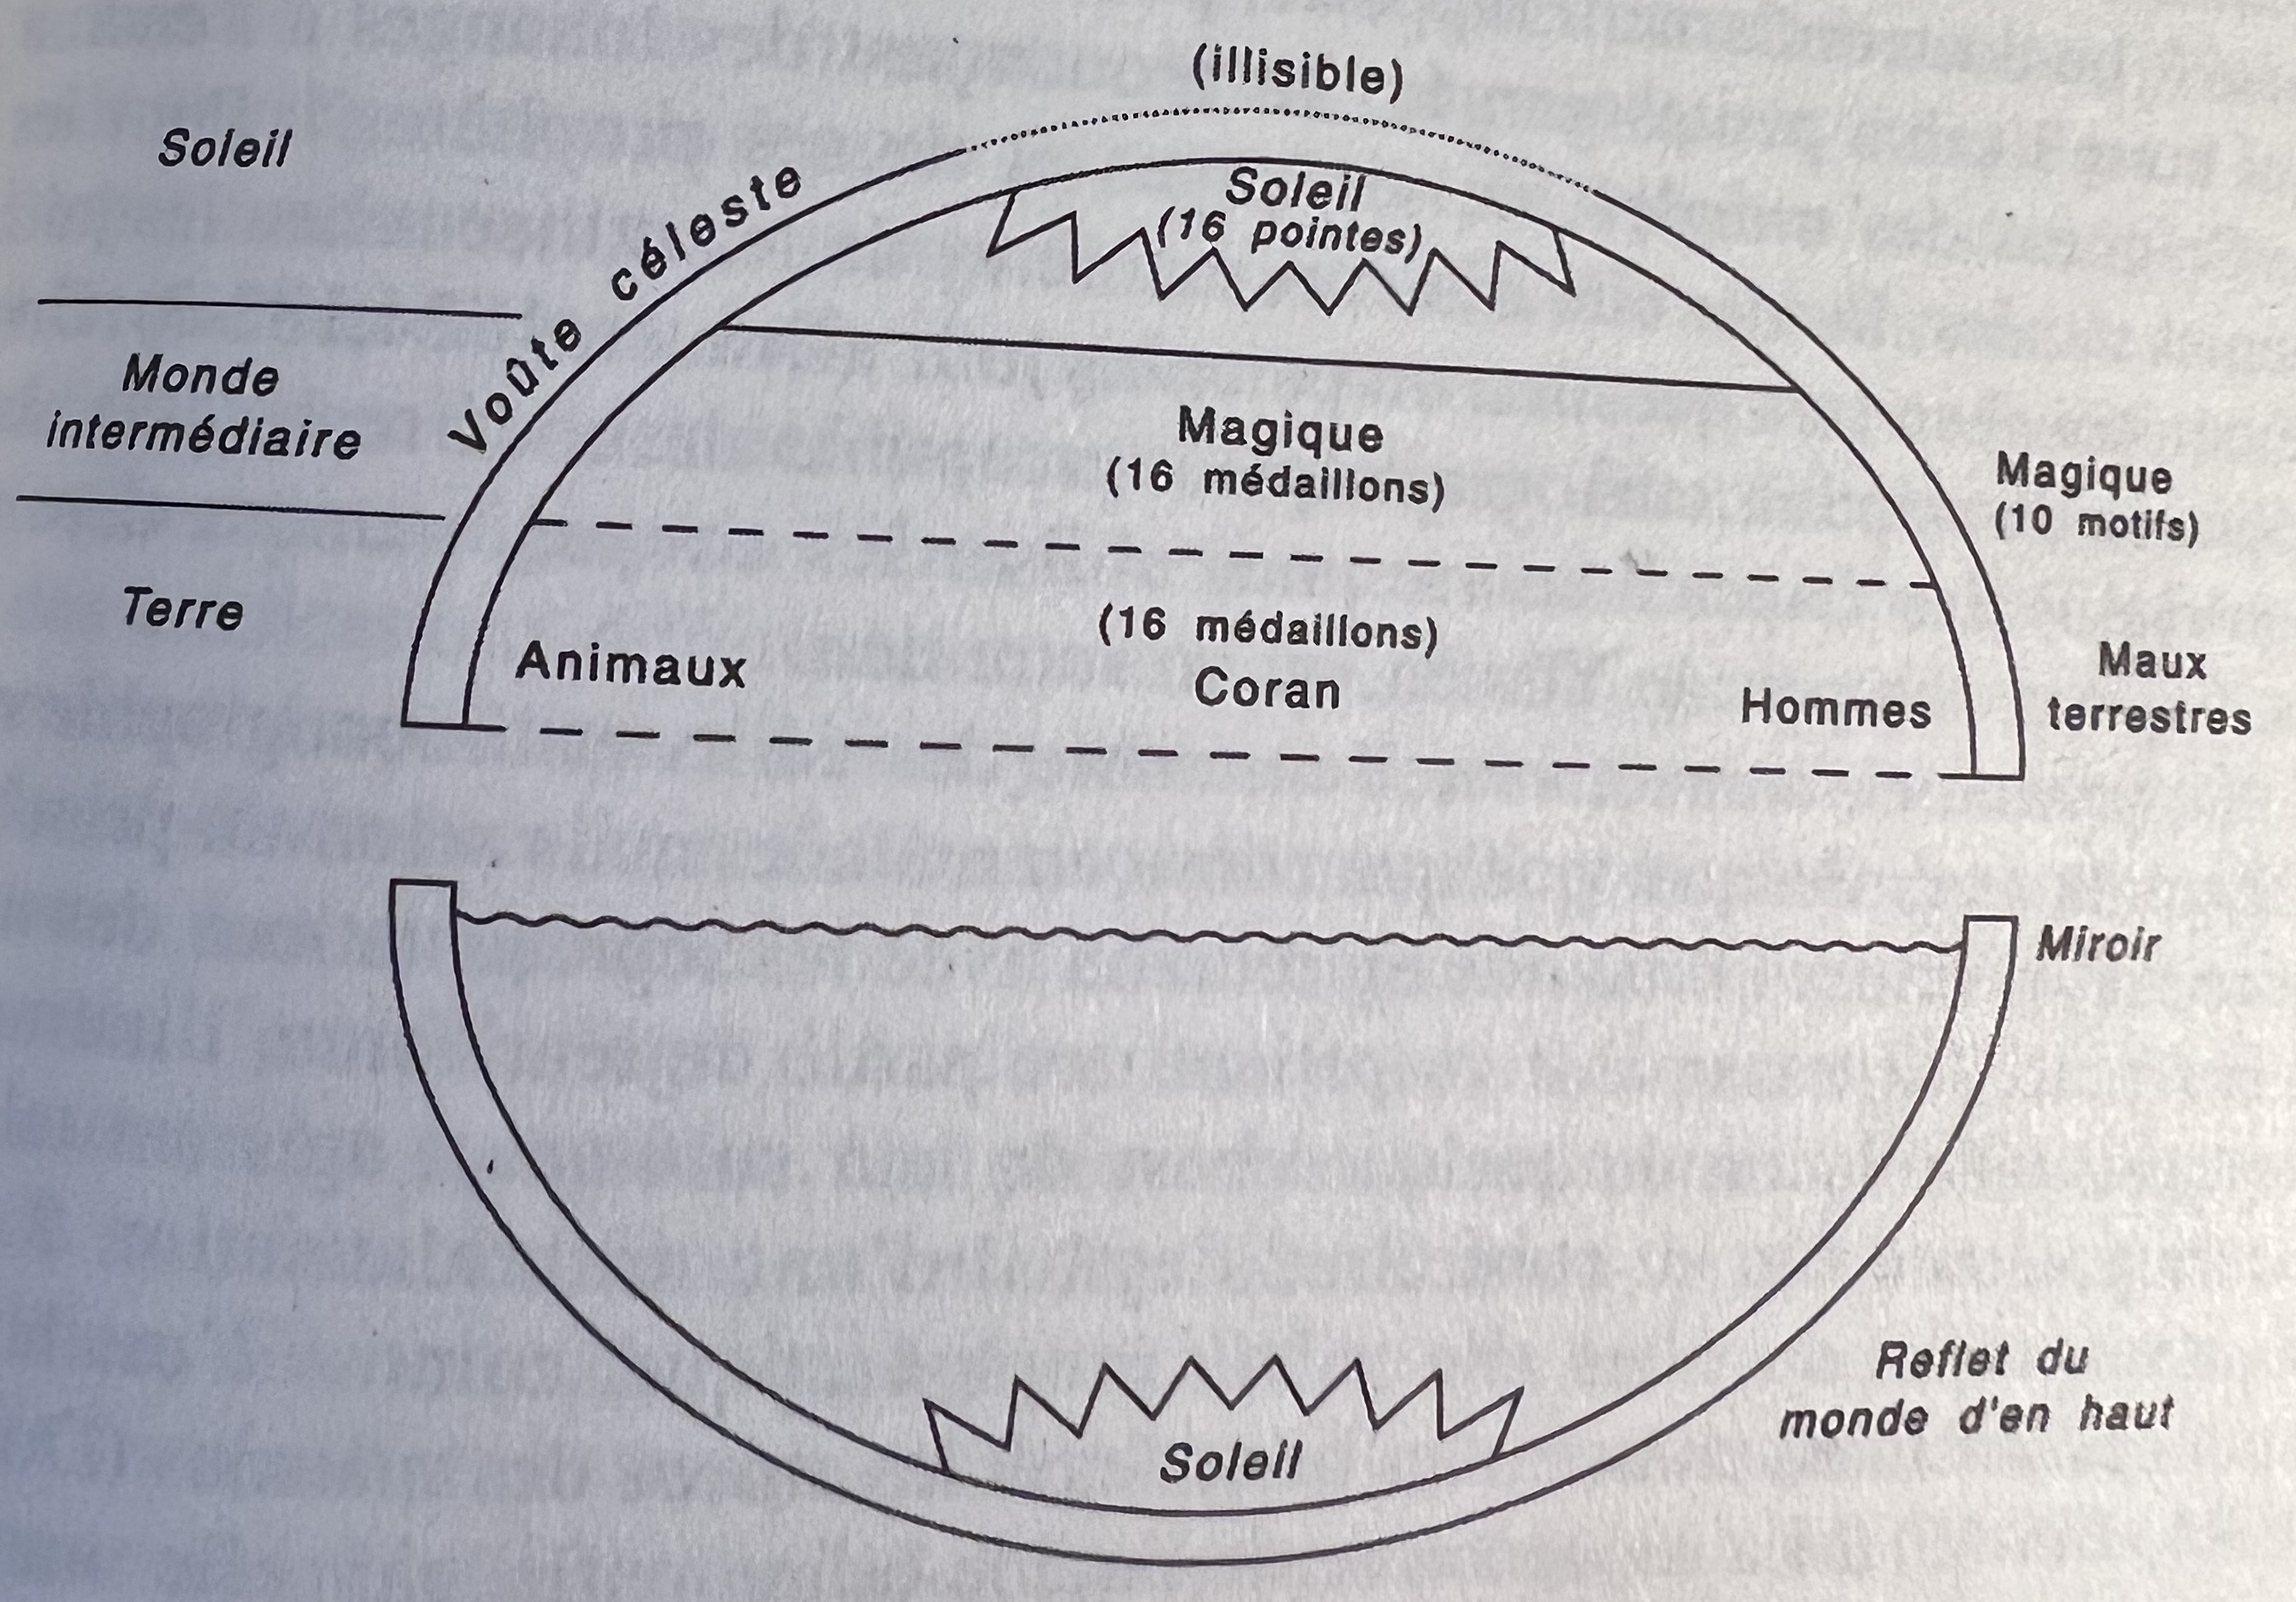
\includegraphics[width=0.7\textwidth]{HommeetIslam/Images/IMG_2459recadre.png}
   \caption{La Coupe comme représentation du cosmos. Coupe B paroi Interne et externe}
    \label{fig:my_label}
\end{figure}
 
\subsection*{Des biens d'une fondation pieuse - \textit{waqf}}
Après avoir étudié la coupe proprement dite, l'auteure étudie le statut particulier de ces coupes : elles sont la propriété d'une fondation pieuse, \textit{waqf}, depuis 1895. Pratiquement, il s'agit d'un \textit{waqf} oral, non enregistré auprès des autorités à la différence des biens immobiliers.
En étant \textit{waqf}, la légitimité religieuse est
renforcée. 
Mais ce qui retient l'attention, c'est le faible empressement de l'intendant de la mosquée envers les 2 coupes, dont il est pourtant le gestionnaire. Il les prête gratuitement quand on les lui demande mais il peut même douter de leur efficacité. Le pouvoir magique ne vient donc pas du propriétaire et de ses références magiques (à aucun moment la compétence magique n'est requise pour être responsable de mosquée) mais bien des coupes elles-mêmes,  du rite autour de ces coupes, ou de l'artisan qui les a fabriquées. Ceci est confirmé par le fait que de telles coupes étaient offertes en cadeau, au retour du pèlerinage à La Mecque (Canaan 1923, 130 \cite[note 63]{Regourd_2007}); la coupe (A) aurait ainsi été donnée en \textit{waqf} par un \textit{hâjjî}.

\subsection*{Utilisation des coupes}
L'enquête de terrain permet de décrire l'utilisation de ces coupes, en particulier dans le cas de grossesse difficile. 

\paragraph{Leur mode d’emploi consiste principalement à boire un liquide au contact de la coupe.}  Ce liquide - de
l’eau, du bouillon - ou le miel que l’on y a versé, est bu en disant des louanges à Dieu.
Le bouillon de viande est particulièrement prescrit pour les femmes en couches : par son pouvoir nutritif important (moelle,...), il présente des caractéristiques médicales intéressantes,  qui
viennent en addition de celles des écrits et représentations présents sur les coupes. 
\paragraph{La maladie est interprétée comme la conséquence de causes multiples.} Un tel recours simultané à plusieurs médecines différentes est courant dans la même région du Yémen. Il s'agit d'attaquer le mal dans toutes ses facettes. Lorsqu’il y a maladie,
elle est toujours soupçonnée d’être le résultat de causes multiples et la boisson dans la coupe est envisagée en complément d'autres actions, en fonction du diagnostic thérapeutique. De même, l’utilisation des coupes comme réceptacle de boisson n'est pas envisagée comme l'unique usage des coupes, comme le laisse penser les traces de bougie au fond de la coupe B. 


\subsection*{Historique des coupes}
Une coupe, même abîmée, conserve ses propriétés comme c'est le cas de la coupe B réparée plusieurs fois et qui a perdu une partie de ses écrits; le rite, nous l'avons vu, est des plus simples et ne semble pas complètement fixé. D'où vient donc le pouvoir magique de ces objets ? 

Il nous faut donc étudier l'origine de ces objets, que ce soit leur commanditaire ou l'artisan qui l'a fabriqué.

\paragraph{La titulature de Saladin présente sur les coupes est apocryphe.} Le commanditaire de ces coupes serait Saladin, une titulature clairement apocryphe et commune dans les objets magiques. Par une telle référence, la légitimité du pouvoir magique se trouve renforcée. 

 


\paragraph{Le rôle de l'artisan est secondaire.} Nous n'avons pas d'informations sur l'artisan mais l'étude des diverses coupes magiques montre des artisans différents, certains excellents, d'autres se contentant de copies mais toujours avec des variantes. 
Selon les mentions de certaines coupes, la puissance magique viendrait ou serait renforcée par la survenance d'un évènement astral lors de la fabrication de l'objet. Une telle mention, doublée parfois du nom d'un souverain,  ajoute par sa simple évocation, à la valeur et l'efficacité de la coupe.  
\paragraph{L'homme s'approprie la magie d'origine divine.} Nous avons vu que dans la vision coranique, la magie n'est pas innée pour l'homme.
Un mythe d’origine
des coupes véhicule l’idée que la copie peut avoir autant d’effet que
l’original. Les Palestiniens expliquent
ainsi l'origine des coupes : les bons anges en employaient de semblables
pour faire leurs ablutions. Ils en oublièrent un jour quelques exemplaires
à côté de la source où ils avaient 1'habitude de se rassembler pour se
laver. Un homme passant par là les trouva et s'en empara. Les propriétés
miraculeuses de la coupe furent bientôt découvertes. Des copies en furent
réalisées, qui manifestèrent les mêmes propriétés (Canaan, 1923,130;
1936, 127 cité par \cite{Regourd_2007})

 

 \subsection*{Conclusion}

\paragraph{La source de la magie semble l'addition de plusieurs facteurs } A la fin de cette étude, le pouvoir de ces coupes semble venir de l'addition de plusieurs facteurs et non d'un seul : mythe originel lié aux anges, titulature de Saladin, caractères magiques, formules coraniques adaptées, animaux et sceaux de Salomon, bien \textit{waqf}. 
De la même façon, son utilisation sera complétée d'autres approches thérapeutiques pour une approche que l'on qualifierait aujourd'hui d'\textit{holistique}.

\paragraph{L'anthropologie éclaire l'islamologie} En guise de conclusion, nous essayons de penser les conséquences de cette recherche anthropologique pour l'islamologie. Il apparaît de l'étude des diverses coupes que la magie n'est pas uniquement un élément exogène ajouté  à la foi musulmane mais fait du Coran une réalité bien plus riche qu'un simple livre à lire et à étudier, avec une lecture littérale du verset  : 
\begin{quote}
    Nous envoyons du Coran ce qui est une guérison et une miséricorde pour les croyants. (17:82)
\end{quote}
\vspace{1cm}
Développant ce verset, Winter peut conclure : 
\begin{singlequote}
    This healing
power of the revelation is understood literally by many, not just spiritually.
The qur’an was thus sometimes also used physically for curing [\ldots]. By means of amulets,
talismanic shirts and other artefacts covered with qur’anic inscriptions, often
in conjunction with astrological or magical devices or practices, the revelation
came to be put to all kinds of uses, not always strictly orthodox. By procedures reminiscent of the Cabbala, the letters of the Arabic alphabet and their
numerical values themselves played an important role in Muslim mysticism,
esotericism and the divinatory arts. \cite{winter_cambridge_2008}
\end{singlequote}
 
 
 